\documentclass[]{article}
\usepackage{lmodern}
\usepackage{amssymb,amsmath}
\usepackage{ifxetex,ifluatex}
\usepackage{fixltx2e} % provides \textsubscript
\ifnum 0\ifxetex 1\fi\ifluatex 1\fi=0 % if pdftex
  \usepackage[T1]{fontenc}
  \usepackage[utf8]{inputenc}
\else % if luatex or xelatex
  \ifxetex
    \usepackage{mathspec}
  \else
    \usepackage{fontspec}
  \fi
  \defaultfontfeatures{Ligatures=TeX,Scale=MatchLowercase}
\fi
% use upquote if available, for straight quotes in verbatim environments
\IfFileExists{upquote.sty}{\usepackage{upquote}}{}
% use microtype if available
\IfFileExists{microtype.sty}{%
\usepackage{microtype}
\UseMicrotypeSet[protrusion]{basicmath} % disable protrusion for tt fonts
}{}
\usepackage[margin=1in]{geometry}
\usepackage{hyperref}
\hypersetup{unicode=true,
            pdftitle={Movielens},
            pdfborder={0 0 0},
            breaklinks=true}
\urlstyle{same}  % don't use monospace font for urls
\usepackage{color}
\usepackage{fancyvrb}
\newcommand{\VerbBar}{|}
\newcommand{\VERB}{\Verb[commandchars=\\\{\}]}
\DefineVerbatimEnvironment{Highlighting}{Verbatim}{commandchars=\\\{\}}
% Add ',fontsize=\small' for more characters per line
\usepackage{framed}
\definecolor{shadecolor}{RGB}{248,248,248}
\newenvironment{Shaded}{\begin{snugshade}}{\end{snugshade}}
\newcommand{\AlertTok}[1]{\textcolor[rgb]{0.94,0.16,0.16}{#1}}
\newcommand{\AnnotationTok}[1]{\textcolor[rgb]{0.56,0.35,0.01}{\textbf{\textit{#1}}}}
\newcommand{\AttributeTok}[1]{\textcolor[rgb]{0.77,0.63,0.00}{#1}}
\newcommand{\BaseNTok}[1]{\textcolor[rgb]{0.00,0.00,0.81}{#1}}
\newcommand{\BuiltInTok}[1]{#1}
\newcommand{\CharTok}[1]{\textcolor[rgb]{0.31,0.60,0.02}{#1}}
\newcommand{\CommentTok}[1]{\textcolor[rgb]{0.56,0.35,0.01}{\textit{#1}}}
\newcommand{\CommentVarTok}[1]{\textcolor[rgb]{0.56,0.35,0.01}{\textbf{\textit{#1}}}}
\newcommand{\ConstantTok}[1]{\textcolor[rgb]{0.00,0.00,0.00}{#1}}
\newcommand{\ControlFlowTok}[1]{\textcolor[rgb]{0.13,0.29,0.53}{\textbf{#1}}}
\newcommand{\DataTypeTok}[1]{\textcolor[rgb]{0.13,0.29,0.53}{#1}}
\newcommand{\DecValTok}[1]{\textcolor[rgb]{0.00,0.00,0.81}{#1}}
\newcommand{\DocumentationTok}[1]{\textcolor[rgb]{0.56,0.35,0.01}{\textbf{\textit{#1}}}}
\newcommand{\ErrorTok}[1]{\textcolor[rgb]{0.64,0.00,0.00}{\textbf{#1}}}
\newcommand{\ExtensionTok}[1]{#1}
\newcommand{\FloatTok}[1]{\textcolor[rgb]{0.00,0.00,0.81}{#1}}
\newcommand{\FunctionTok}[1]{\textcolor[rgb]{0.00,0.00,0.00}{#1}}
\newcommand{\ImportTok}[1]{#1}
\newcommand{\InformationTok}[1]{\textcolor[rgb]{0.56,0.35,0.01}{\textbf{\textit{#1}}}}
\newcommand{\KeywordTok}[1]{\textcolor[rgb]{0.13,0.29,0.53}{\textbf{#1}}}
\newcommand{\NormalTok}[1]{#1}
\newcommand{\OperatorTok}[1]{\textcolor[rgb]{0.81,0.36,0.00}{\textbf{#1}}}
\newcommand{\OtherTok}[1]{\textcolor[rgb]{0.56,0.35,0.01}{#1}}
\newcommand{\PreprocessorTok}[1]{\textcolor[rgb]{0.56,0.35,0.01}{\textit{#1}}}
\newcommand{\RegionMarkerTok}[1]{#1}
\newcommand{\SpecialCharTok}[1]{\textcolor[rgb]{0.00,0.00,0.00}{#1}}
\newcommand{\SpecialStringTok}[1]{\textcolor[rgb]{0.31,0.60,0.02}{#1}}
\newcommand{\StringTok}[1]{\textcolor[rgb]{0.31,0.60,0.02}{#1}}
\newcommand{\VariableTok}[1]{\textcolor[rgb]{0.00,0.00,0.00}{#1}}
\newcommand{\VerbatimStringTok}[1]{\textcolor[rgb]{0.31,0.60,0.02}{#1}}
\newcommand{\WarningTok}[1]{\textcolor[rgb]{0.56,0.35,0.01}{\textbf{\textit{#1}}}}
\usepackage{longtable,booktabs}
\usepackage{graphicx,grffile}
\makeatletter
\def\maxwidth{\ifdim\Gin@nat@width>\linewidth\linewidth\else\Gin@nat@width\fi}
\def\maxheight{\ifdim\Gin@nat@height>\textheight\textheight\else\Gin@nat@height\fi}
\makeatother
% Scale images if necessary, so that they will not overflow the page
% margins by default, and it is still possible to overwrite the defaults
% using explicit options in \includegraphics[width, height, ...]{}
\setkeys{Gin}{width=\maxwidth,height=\maxheight,keepaspectratio}
\IfFileExists{parskip.sty}{%
\usepackage{parskip}
}{% else
\setlength{\parindent}{0pt}
\setlength{\parskip}{6pt plus 2pt minus 1pt}
}
\setlength{\emergencystretch}{3em}  % prevent overfull lines
\providecommand{\tightlist}{%
  \setlength{\itemsep}{0pt}\setlength{\parskip}{0pt}}
\setcounter{secnumdepth}{0}
% Redefines (sub)paragraphs to behave more like sections
\ifx\paragraph\undefined\else
\let\oldparagraph\paragraph
\renewcommand{\paragraph}[1]{\oldparagraph{#1}\mbox{}}
\fi
\ifx\subparagraph\undefined\else
\let\oldsubparagraph\subparagraph
\renewcommand{\subparagraph}[1]{\oldsubparagraph{#1}\mbox{}}
\fi

%%% Use protect on footnotes to avoid problems with footnotes in titles
\let\rmarkdownfootnote\footnote%
\def\footnote{\protect\rmarkdownfootnote}

%%% Change title format to be more compact
\usepackage{titling}

% Create subtitle command for use in maketitle
\providecommand{\subtitle}[1]{
  \posttitle{
    \begin{center}\large#1\end{center}
    }
}

\setlength{\droptitle}{-2em}

  \title{Movielens}
    \pretitle{\vspace{\droptitle}\centering\huge}
  \posttitle{\par}
    \author{}
    \preauthor{}\postauthor{}
      \predate{\centering\large\emph}
  \postdate{\par}
    \date{2019-06-19 17:09:37}


\begin{document}
\maketitle

{
\setcounter{tocdepth}{3}
\tableofcontents
}
\hypertarget{load-and-preview-data}{%
\section{Load and preview data}\label{load-and-preview-data}}

Read data from the \texttt{ratings.csv} file

\begin{Shaded}
\begin{Highlighting}[]
\NormalTok{ratings <-}\StringTok{ }\KeywordTok{read_csv}\NormalTok{(}\StringTok{'ratings.csv'}\NormalTok{,}
                    \DataTypeTok{col_names =} \KeywordTok{c}\NormalTok{(}\StringTok{'user_id'}\NormalTok{,}\StringTok{'movie_id'}\NormalTok{,}\StringTok{'rating'}\NormalTok{,}\StringTok{'timestamp'}\NormalTok{))}
\end{Highlighting}
\end{Shaded}

\begin{verbatim}
## Parsed with column specification:
## cols(
##   user_id = col_double(),
##   movie_id = col_double(),
##   rating = col_double(),
##   timestamp = col_double()
## )
\end{verbatim}

Loaded 305.2 Mb of ratings data, containing 10,000,054 ratings. Here's a
preview:

\begin{Shaded}
\begin{Highlighting}[]
\KeywordTok{head}\NormalTok{(ratings) }\OperatorTok\StringTok{ }\KeywordTok{kable}\NormalTok{()}
\end{Highlighting}
\end{Shaded}

\begin{longtable}[]{@{}rrrr@{}}
\toprule
user\_id & movie\_id & rating & timestamp\tabularnewline
\midrule
\endhead
1 & 122 & 5 & 838985046\tabularnewline
1 & 185 & 5 & 838983525\tabularnewline
1 & 231 & 5 & 838983392\tabularnewline
1 & 292 & 5 & 838983421\tabularnewline
1 & 316 & 5 & 838983392\tabularnewline
1 & 329 & 5 & 838983392\tabularnewline
\bottomrule
\end{longtable}

\hypertarget{summary-statistics}{%
\section{Summary statistics}\label{summary-statistics}}

\begin{Shaded}
\begin{Highlighting}[]
\CommentTok{# plot the distribution of rating values (slide 21)}

\NormalTok{dist_ratings <-}\StringTok{ }\NormalTok{ratings }\OperatorTok\StringTok{ }
\StringTok{  }\KeywordTok{ggplot}\NormalTok{(}\KeywordTok{aes}\NormalTok{( }\DataTypeTok{x =}\NormalTok{ rating)) }\OperatorTok{+}
\StringTok{  }\KeywordTok{geom_histogram}\NormalTok{(}\DataTypeTok{bins =} \DecValTok{30}\NormalTok{, }\DataTypeTok{fill =} \StringTok{"blue"}\NormalTok{) }\OperatorTok{+}
\StringTok{  }\KeywordTok{labs}\NormalTok{(}\DataTypeTok{x =} \StringTok{"Rating"}\NormalTok{, }\DataTypeTok{y =} \StringTok{"Number of ratings"}\NormalTok{, }\DataTypeTok{title =} \StringTok{"Distribution of ratings"}\NormalTok{)}

\KeywordTok{plot}\NormalTok{(dist_ratings)}
\end{Highlighting}
\end{Shaded}

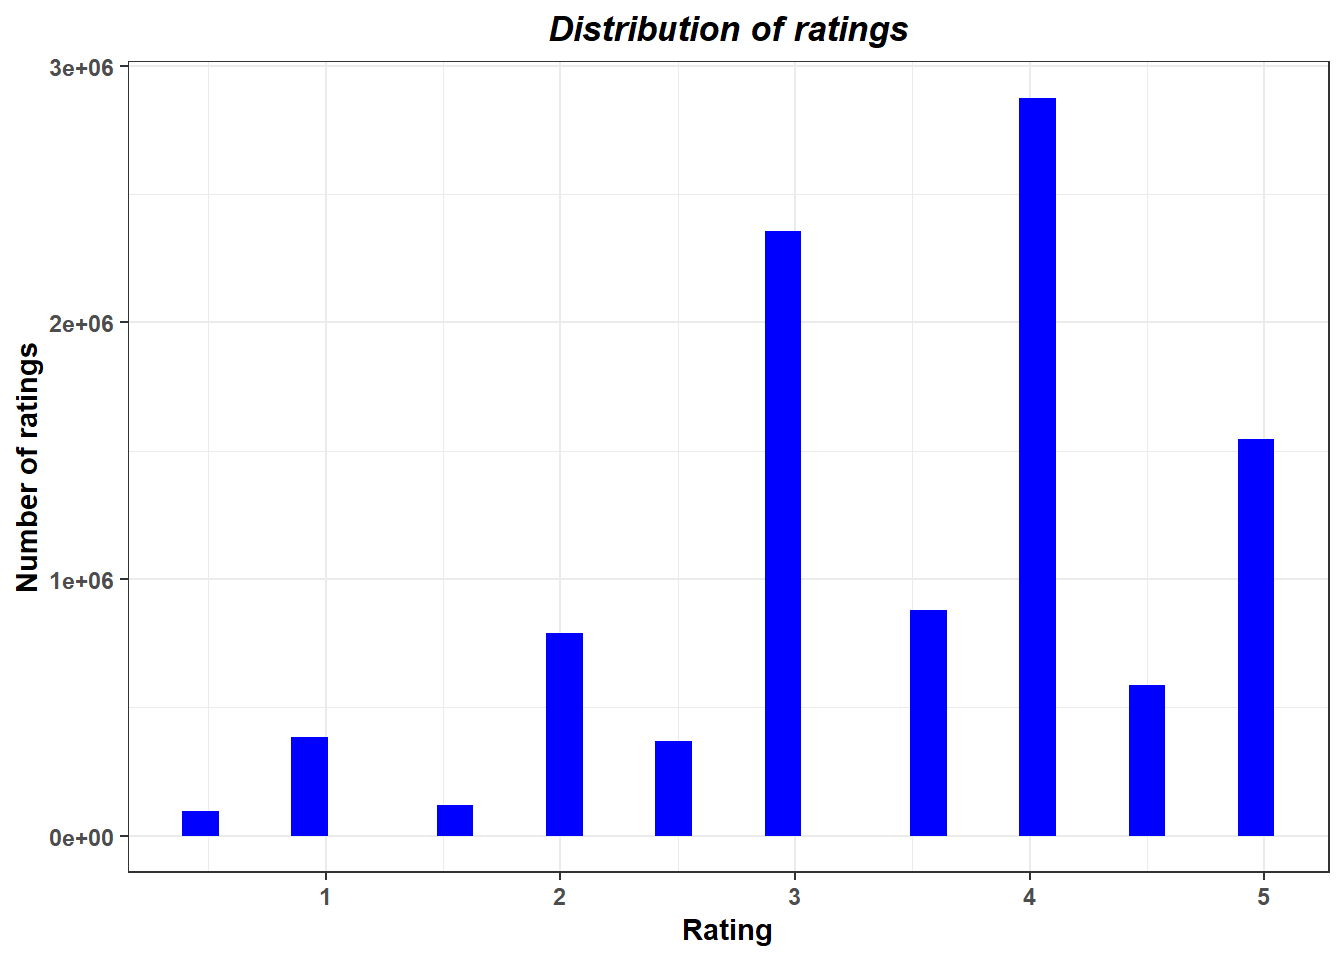
\includegraphics{movielens_files/figure-latex/dist-ratings-1.pdf}

\hypertarget{per-movie-stats}{%
\subsection{Per-movie stats}\label{per-movie-stats}}

\begin{Shaded}
\begin{Highlighting}[]
\CommentTok{# aggregate ratings by movie, computing mean and number of ratings}
\CommentTok{# hint: use the n() function for easy counting within a group}

\NormalTok{aggregate_by_movie <-}\StringTok{ }\NormalTok{ratings }\OperatorTok\StringTok{ }
\StringTok{  }\KeywordTok{group_by}\NormalTok{(movie_id) }\OperatorTok
\StringTok{  }\KeywordTok{summarize}\NormalTok{(}\DataTypeTok{count =} \KeywordTok{n}\NormalTok{(), }\DataTypeTok{avg_rating =} \KeywordTok{mean}\NormalTok{(rating))}

\KeywordTok{View}\NormalTok{(aggregate_by_movie)}
\end{Highlighting}
\end{Shaded}

\begin{Shaded}
\begin{Highlighting}[]
\CommentTok{# plot distribution of movie popularity (= number of ratings the movie received)}
\CommentTok{# hint: try scale_x_log10() for a logarithmic x axis}

\NormalTok{dist_movie_pop <-}\StringTok{ }\NormalTok{ratings }\OperatorTok\StringTok{ }
\StringTok{  }\KeywordTok{group_by}\NormalTok{(movie_id) }\OperatorTok
\StringTok{  }\KeywordTok{summarize}\NormalTok{(}\DataTypeTok{count =} \KeywordTok{n}\NormalTok{()) }\OperatorTok\StringTok{ }
\StringTok{  }\KeywordTok{ungroup}\NormalTok{() }\OperatorTok
\StringTok{  }\KeywordTok{ggplot}\NormalTok{(}\KeywordTok{aes}\NormalTok{(}\DataTypeTok{x =}\NormalTok{ count)) }\OperatorTok{+}
\StringTok{  }\KeywordTok{geom_histogram}\NormalTok{(}\DataTypeTok{bins =} \DecValTok{30}\NormalTok{, }\DataTypeTok{fill =} \StringTok{"gray"}\NormalTok{, }\DataTypeTok{color =} \StringTok{"black"}\NormalTok{) }\OperatorTok{+}\StringTok{ }
\StringTok{  }\KeywordTok{scale_x_log10}\NormalTok{(}\DataTypeTok{label =}\NormalTok{ comma) }\OperatorTok{+}
\StringTok{  }\KeywordTok{labs}\NormalTok{(}\DataTypeTok{x =} \StringTok{"Number of rating"}\NormalTok{, }\DataTypeTok{y =} \StringTok{"Number of movies"}\NormalTok{, }\DataTypeTok{title =} \StringTok{"Distribution of Movie Popularity"}\NormalTok{) }

\KeywordTok{plot}\NormalTok{(dist_movie_pop)}
\end{Highlighting}
\end{Shaded}

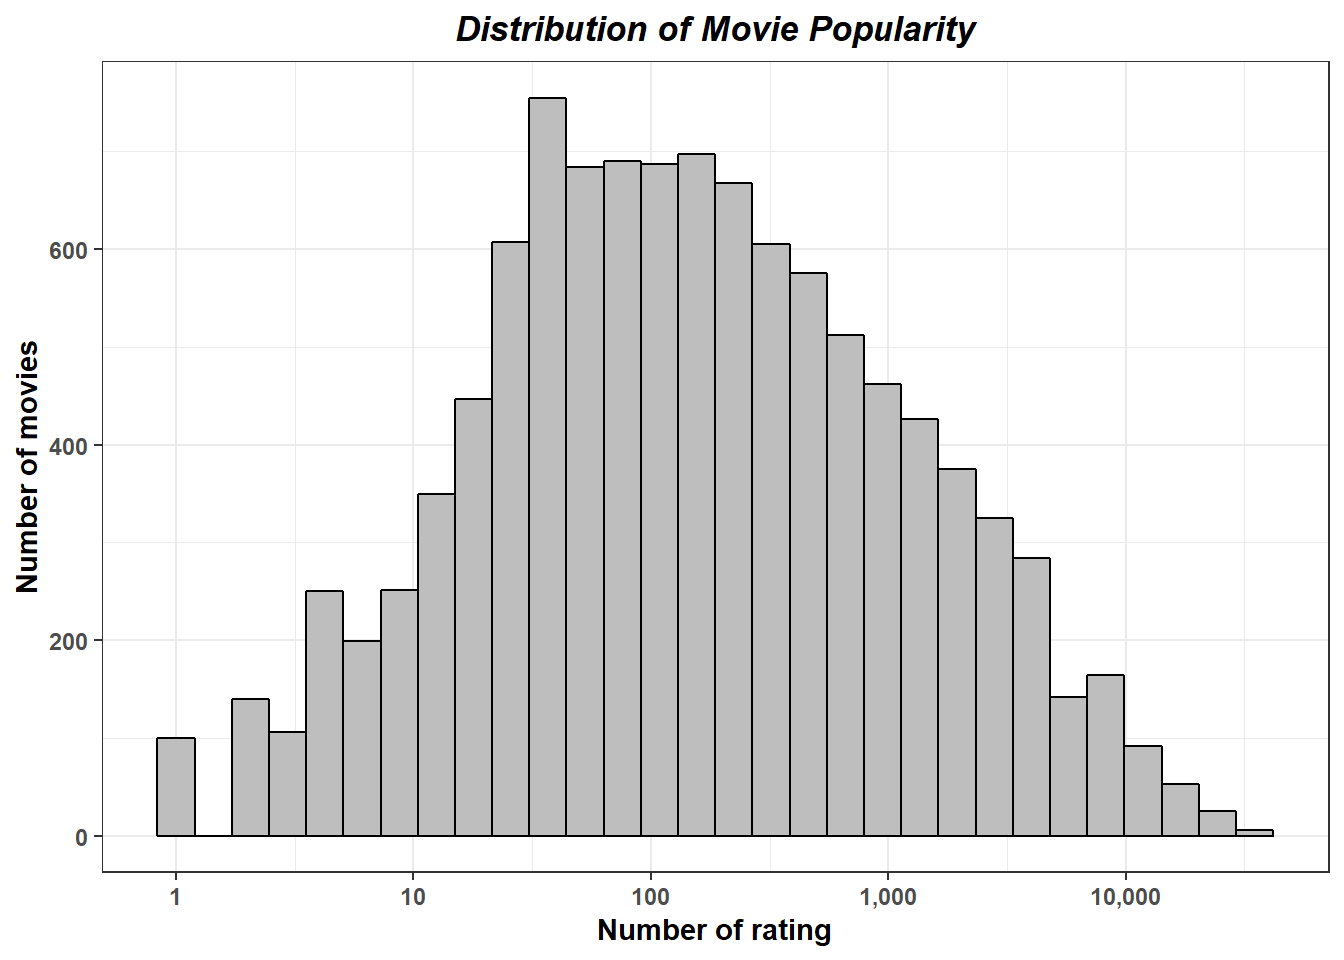
\includegraphics{movielens_files/figure-latex/dist-movie-popularity-1.pdf}

\begin{Shaded}
\begin{Highlighting}[]
\CommentTok{# plot distribution of mean ratings by movie (slide 23)}
\CommentTok{# hint: try geom_histogram and geom_density}

\NormalTok{dist_mean_ratings_by_movie <-}\StringTok{ }\NormalTok{ratings }\OperatorTok\StringTok{ }
\StringTok{  }\KeywordTok{group_by}\NormalTok{(movie_id) }\OperatorTok\StringTok{ }
\StringTok{  }\KeywordTok{summarize}\NormalTok{(}\DataTypeTok{count =} \KeywordTok{n}\NormalTok{(), }\DataTypeTok{mean_rating =} \KeywordTok{mean}\NormalTok{(rating)) }\OperatorTok\StringTok{ }
\StringTok{  }\KeywordTok{ungroup}\NormalTok{() }\OperatorTok\StringTok{ }
\StringTok{  }\KeywordTok{ggplot}\NormalTok{(}\KeywordTok{aes}\NormalTok{( }\DataTypeTok{x =}\NormalTok{ mean_rating)) }\OperatorTok{+}
\StringTok{  }\KeywordTok{geom_histogram}\NormalTok{(}\DataTypeTok{bins =} \DecValTok{30}\NormalTok{, }\DataTypeTok{fill =} \StringTok{"gray"}\NormalTok{, }\DataTypeTok{color =} \StringTok{"black"}\NormalTok{) }\OperatorTok{+}
\StringTok{  }\KeywordTok{geom_density}\NormalTok{() }\OperatorTok{+}
\StringTok{  }\KeywordTok{labs}\NormalTok{(}\DataTypeTok{x =} \StringTok{"Average Rating"}\NormalTok{, }\DataTypeTok{y =} \StringTok{"Number of Movie"}\NormalTok{, }\DataTypeTok{title =} \StringTok{"Distribution of Mean-ratings by Movie"}\NormalTok{)}

\NormalTok{dist_mean_ratings_by_movie }\OperatorTok\StringTok{ }\KeywordTok{plot}\NormalTok{()}
\end{Highlighting}
\end{Shaded}

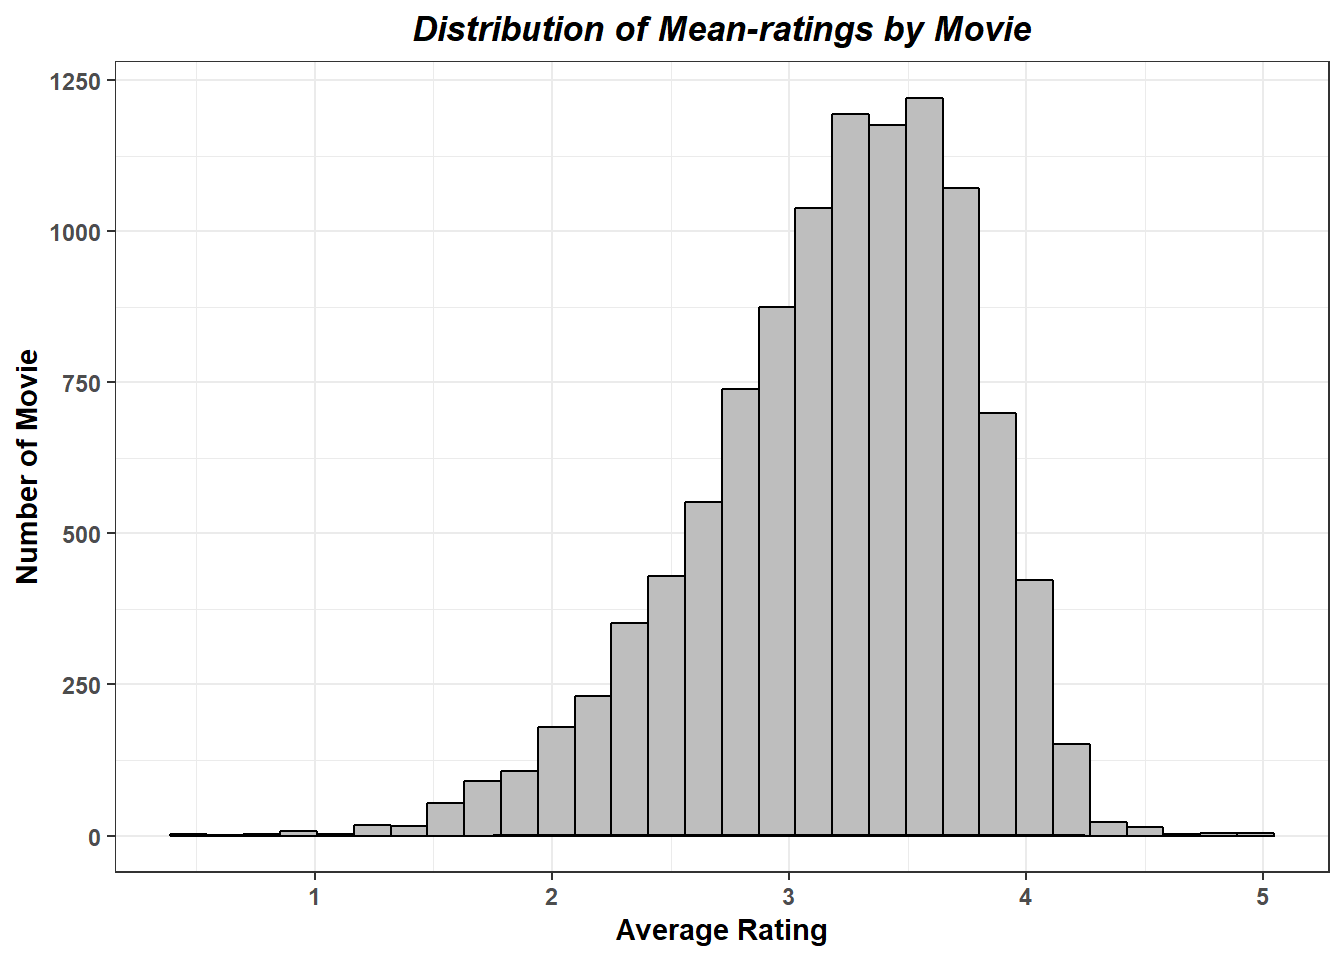
\includegraphics{movielens_files/figure-latex/dist-mean-ratings-by-movie-1.pdf}

\begin{Shaded}
\begin{Highlighting}[]
\CommentTok{# rank movies by popularity and compute the cdf, or fraction of movies covered by the top-k moves (slide 25)}
\CommentTok{# hint: use dplyr's rank and arrange functions, and the base R sum and cumsum functions}
\CommentTok{# store the result in a new data frame so you can use it in creating figure 2 from the paper below}

\CommentTok{# plot the CDF of movie popularity}

\NormalTok{cdf_movie_pop <-}\StringTok{ }\NormalTok{ratings }\OperatorTok
\StringTok{  }\KeywordTok{group_by}\NormalTok{(movie_id) }\OperatorTok\StringTok{ }
\StringTok{  }\KeywordTok{summarize}\NormalTok{(}\DataTypeTok{count =} \KeywordTok{n}\NormalTok{()) }\OperatorTok
\StringTok{  }\KeywordTok{arrange}\NormalTok{(}\KeywordTok{desc}\NormalTok{(count)) }\OperatorTok\StringTok{ }
\StringTok{  }\KeywordTok{mutate}\NormalTok{(}\DataTypeTok{rank =} \KeywordTok{rank}\NormalTok{(}\KeywordTok{desc}\NormalTok{(count)),}
         \DataTypeTok{frac_ratings =} \KeywordTok{cumsum}\NormalTok{(count) }\OperatorTok{/}\StringTok{ }\KeywordTok{sum}\NormalTok{(count)) }\OperatorTok
\StringTok{  }\KeywordTok{ungroup}\NormalTok{()}

\CommentTok{# View(cdf_movie_pop)}

\NormalTok{cdf_movie_pop }\OperatorTok\StringTok{ }
\StringTok{  }\KeywordTok{ggplot}\NormalTok{(}\KeywordTok{aes}\NormalTok{(}\DataTypeTok{x =}\NormalTok{ rank, }\DataTypeTok{y =}\NormalTok{ frac_ratings)) }\OperatorTok{+}
\StringTok{  }\KeywordTok{geom_line}\NormalTok{() }\OperatorTok{+}
\StringTok{  }\KeywordTok{labs}\NormalTok{(}\DataTypeTok{x =} \StringTok{"Rank"}\NormalTok{, }\DataTypeTok{y =} \StringTok{"CDF"}\NormalTok{, }
       \DataTypeTok{title =} \StringTok{"Long Tail Analogy"}\NormalTok{)}
\end{Highlighting}
\end{Shaded}

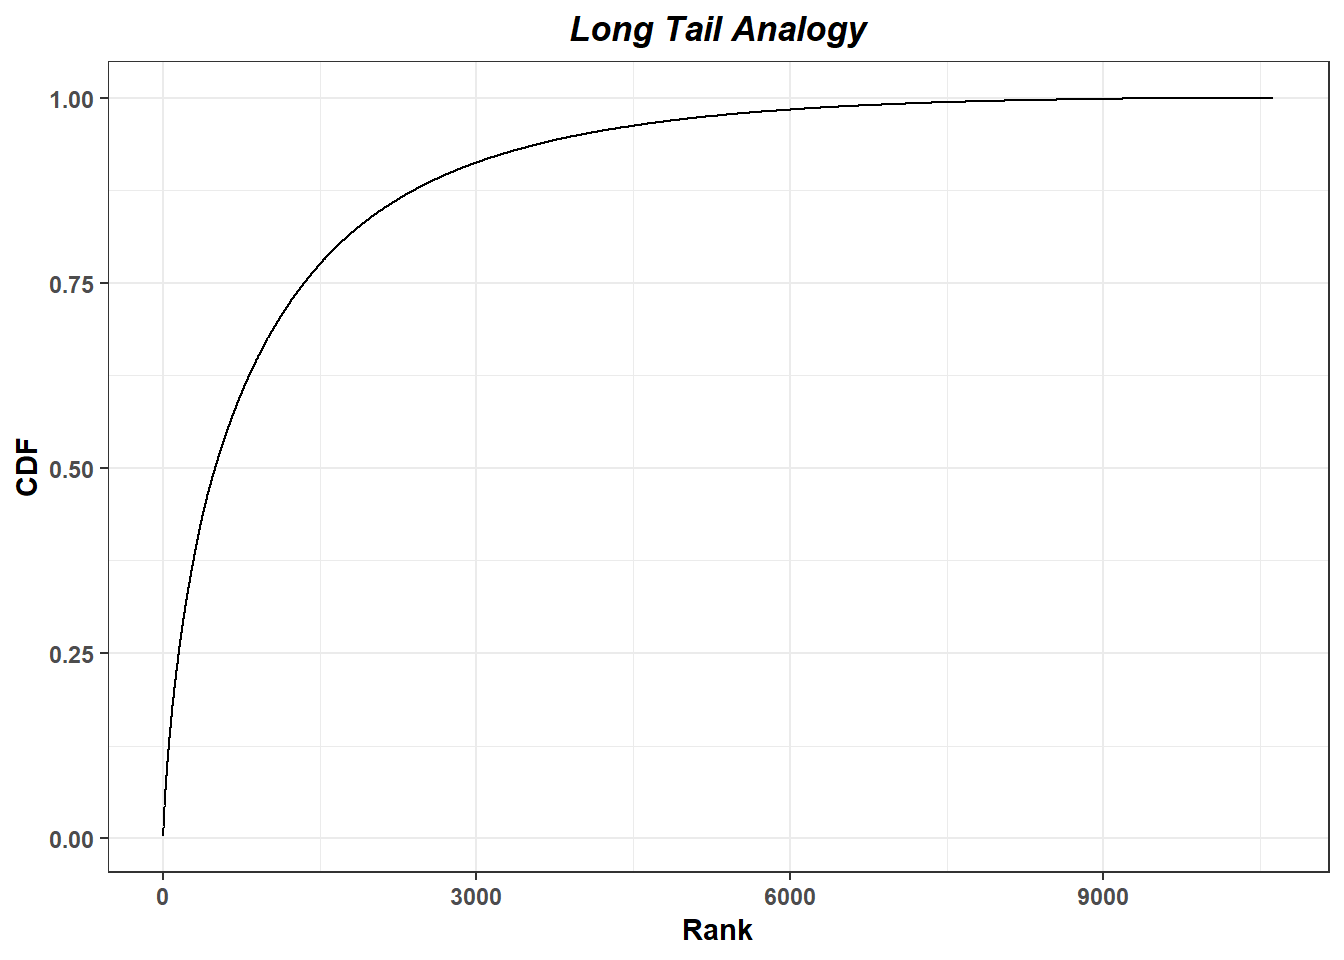
\includegraphics{movielens_files/figure-latex/cdf-movie-pop-1.pdf}

\hypertarget{per-user-stats}{%
\section{Per-user stats}\label{per-user-stats}}

\begin{Shaded}
\begin{Highlighting}[]
\CommentTok{# aggregate ratings by user, computing mean and number of ratings}

\NormalTok{aggregate_by_user <-}\StringTok{ }\NormalTok{ratings }\OperatorTok
\StringTok{  }\KeywordTok{group_by}\NormalTok{(user_id) }\OperatorTok\StringTok{ }
\StringTok{  }\KeywordTok{summarize}\NormalTok{(}\DataTypeTok{count =} \KeywordTok{n}\NormalTok{(), }\DataTypeTok{mean =} \KeywordTok{mean}\NormalTok{(rating)) }\OperatorTok\StringTok{ }
\StringTok{  }\KeywordTok{arrange}\NormalTok{(}\KeywordTok{desc}\NormalTok{(count)) }\OperatorTok\StringTok{ }
\StringTok{  }\KeywordTok{ungroup}\NormalTok{()}

  \KeywordTok{View}\NormalTok{(aggregate_by_user)}
\end{Highlighting}
\end{Shaded}

\begin{Shaded}
\begin{Highlighting}[]
\CommentTok{# plot distribution of user activity (= number of ratings the user made)}
\CommentTok{# hint: try a log scale here}

\NormalTok{dist_user_activity <-}\StringTok{ }\NormalTok{aggregate_by_user }\OperatorTok\StringTok{ }
\StringTok{  }\CommentTok{# filter( count >= 10) %>% }
\StringTok{  }\KeywordTok{ggplot}\NormalTok{(}\KeywordTok{aes}\NormalTok{(}\DataTypeTok{x =}\NormalTok{ count, }\DataTypeTok{y =}\NormalTok{ mean)) }\OperatorTok{+}
\StringTok{  }\KeywordTok{geom_point}\NormalTok{() }\OperatorTok{+}
\StringTok{  }\KeywordTok{scale_x_log10}\NormalTok{(}\DataTypeTok{label =}\NormalTok{ comma) }\OperatorTok{+}
\StringTok{  }\KeywordTok{labs}\NormalTok{(}\DataTypeTok{x =} \StringTok{"Number of Ratings per User"}\NormalTok{, }\DataTypeTok{y =} \StringTok{"Average Rating"}\NormalTok{, }\DataTypeTok{title =} \StringTok{"User Activity"}\NormalTok{)}
  

\NormalTok{dist_user_activity }\OperatorTok\StringTok{ }\KeywordTok{plot}\NormalTok{()}
\end{Highlighting}
\end{Shaded}

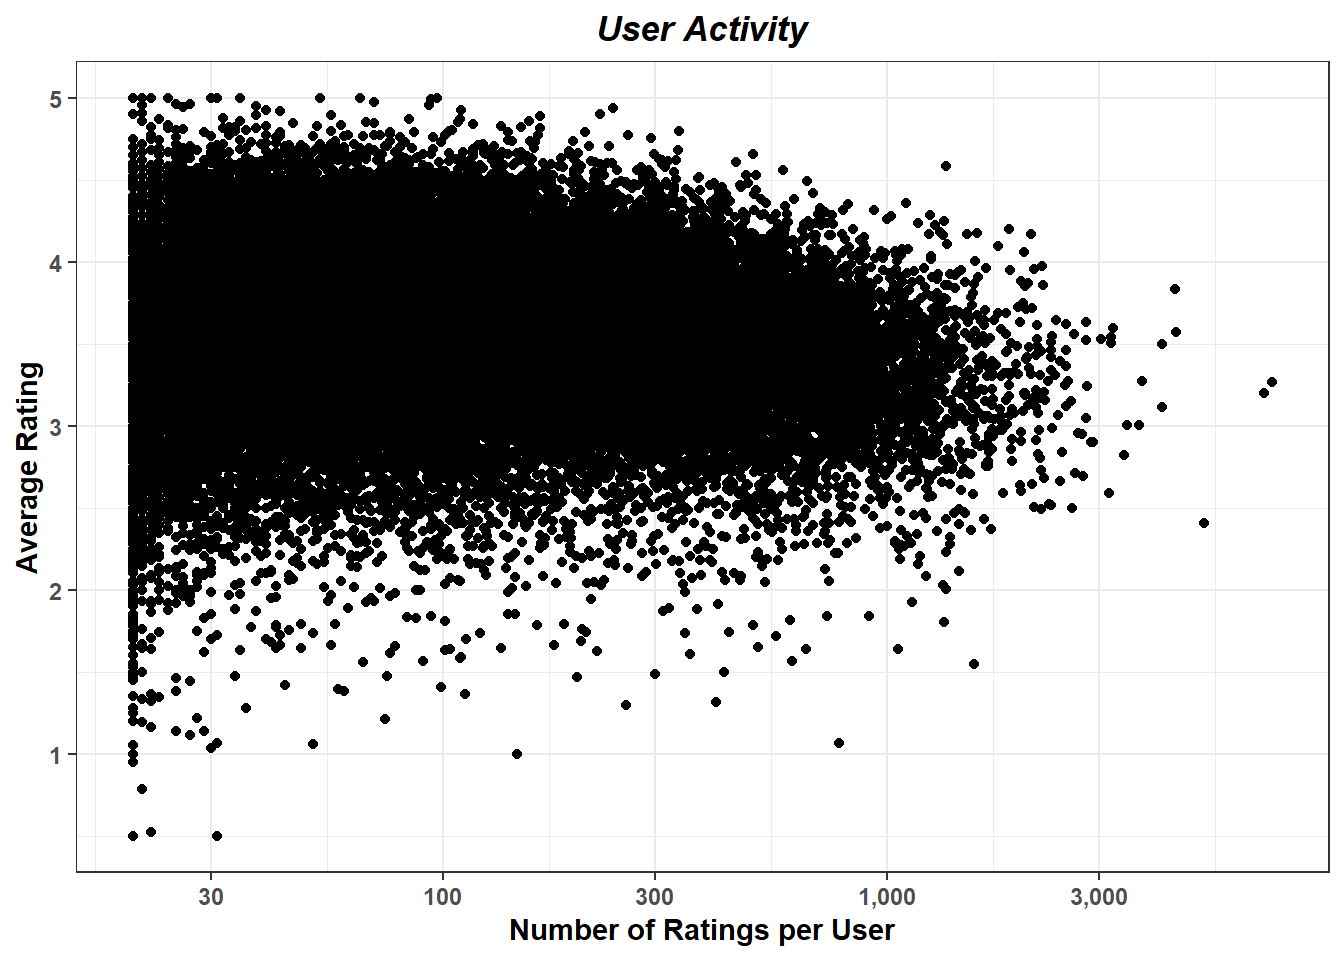
\includegraphics{movielens_files/figure-latex/dist-user-activity-1.pdf}

\hypertarget{anatomy-of-the-long-tail}{%
\section{Anatomy of the long tail}\label{anatomy-of-the-long-tail}}

\begin{Shaded}
\begin{Highlighting}[]
\CommentTok{# generate the equivalent of figure 2 of this paper:}
\CommentTok{# https://5harad.com/papers/long_tail.pdf}

\CommentTok{# Specifically, for the subset of users who rated at least 10 movies,}
\CommentTok{# produce a plot that shows the fraction of users satisfied (vertical}
\CommentTok{# axis) as a function of inventory size (horizontal axis). We will}
\CommentTok{# define "satisfied" as follows: an individual user is satisfied p% of}
\CommentTok{# the time at inventory of size k if at least p% of the movies they}
\CommentTok{# rated are contained in the top k most popular movies. As in the}
\CommentTok{# paper, produce one curve for the 100% user satisfaction level and}
\CommentTok{# another for 90%---do not, however, bother implementing the null}
\CommentTok{# model (shown in the dashed lines).}

\NormalTok{user_rate_}\DecValTok{10}\NormalTok{_plus <-}\StringTok{ }\NormalTok{ratings }\OperatorTok\StringTok{ }
\StringTok{  }\KeywordTok{group_by}\NormalTok{(user_id) }\OperatorTok
\StringTok{  }\KeywordTok{summarise}\NormalTok{(}\DataTypeTok{count =} \KeywordTok{n}\NormalTok{()) }\OperatorTok
\StringTok{  }\KeywordTok{filter}\NormalTok{( count }\OperatorTok{>=}\StringTok{ }\DecValTok{10}\NormalTok{) }\OperatorTok
\StringTok{  }\KeywordTok{ungroup}\NormalTok{()}


\NormalTok{cdf_movie_pop <-}\StringTok{ }\NormalTok{ratings }\OperatorTok
\StringTok{  }\KeywordTok{group_by}\NormalTok{(movie_id) }\OperatorTok\StringTok{ }
\StringTok{  }\KeywordTok{summarize}\NormalTok{(}\DataTypeTok{count =} \KeywordTok{n}\NormalTok{()) }\OperatorTok
\StringTok{  }\KeywordTok{arrange}\NormalTok{(}\KeywordTok{desc}\NormalTok{(count)) }\OperatorTok\StringTok{ }
\StringTok{  }\KeywordTok{mutate}\NormalTok{(}\DataTypeTok{rank =} \KeywordTok{rank}\NormalTok{(}\KeywordTok{desc}\NormalTok{(count))) }\OperatorTok
\StringTok{  }\KeywordTok{ungroup}\NormalTok{()}

\NormalTok{df1 <-}\StringTok{ }\NormalTok{ratings }\OperatorTok\StringTok{ }\KeywordTok{inner_join}\NormalTok{(cdf_movie_pop, }\DataTypeTok{by =} \KeywordTok{c}\NormalTok{(}\StringTok{"movie_id"}\NormalTok{))}

\CommentTok{# df1 %>% View()}

\NormalTok{df2 <-}\StringTok{ }\NormalTok{df1 }\OperatorTok\StringTok{ }\KeywordTok{inner_join}\NormalTok{(user_rate_}\DecValTok{10}\NormalTok{_plus, }\DataTypeTok{by =} \KeywordTok{c}\NormalTok{(}\StringTok{"user_id"}\NormalTok{))}

\NormalTok{inventory_}\DecValTok{90}\NormalTok{_p <-}\StringTok{ }\NormalTok{df2 }\OperatorTok
\StringTok{  }\KeywordTok{group_by}\NormalTok{(user_id) }\OperatorTok
\StringTok{  }\KeywordTok{summarize}\NormalTok{(}\DataTypeTok{inventory =} \KeywordTok{quantile}\NormalTok{(rank, }\FloatTok{.9}\NormalTok{)) }\OperatorTok
\StringTok{  }\KeywordTok{ungroup}\NormalTok{() }\OperatorTok\StringTok{ }
\StringTok{  }\KeywordTok{group_by}\NormalTok{(inventory) }\OperatorTok\StringTok{ }
\StringTok{  }\KeywordTok{summarize}\NormalTok{(}\DataTypeTok{count =} \KeywordTok{n}\NormalTok{()) }\OperatorTok
\StringTok{  }\KeywordTok{arrange}\NormalTok{(inventory) }\OperatorTok\StringTok{ }
\StringTok{  }\KeywordTok{mutate}\NormalTok{(}\DataTypeTok{frac_ratings =} \KeywordTok{cumsum}\NormalTok{(count) }\OperatorTok{/}\StringTok{ }\KeywordTok{sum}\NormalTok{(count)) }\OperatorTok\StringTok{ }
\StringTok{  }\KeywordTok{ungroup}\NormalTok{()}

\NormalTok{inventory_}\DecValTok{100}\NormalTok{_p <-}\StringTok{ }\NormalTok{df2 }\OperatorTok
\StringTok{  }\KeywordTok{group_by}\NormalTok{(user_id) }\OperatorTok
\StringTok{  }\KeywordTok{summarize}\NormalTok{(}\DataTypeTok{inventory =} \KeywordTok{quantile}\NormalTok{(rank, }\DecValTok{1}\NormalTok{)) }\OperatorTok
\StringTok{  }\KeywordTok{ungroup}\NormalTok{() }\OperatorTok\StringTok{ }
\StringTok{  }\KeywordTok{group_by}\NormalTok{(inventory) }\OperatorTok\StringTok{ }
\StringTok{  }\KeywordTok{summarize}\NormalTok{(}\DataTypeTok{count =} \KeywordTok{n}\NormalTok{()) }\OperatorTok
\StringTok{  }\KeywordTok{arrange}\NormalTok{(inventory) }\OperatorTok\StringTok{ }
\StringTok{  }\KeywordTok{mutate}\NormalTok{(}\DataTypeTok{frac_ratings =} \KeywordTok{cumsum}\NormalTok{(count) }\OperatorTok{/}\StringTok{ }\KeywordTok{sum}\NormalTok{(count))}

\KeywordTok{ggplot}\NormalTok{() }\OperatorTok{+}\StringTok{ }
\StringTok{  }\KeywordTok{geom_line}\NormalTok{(}\DataTypeTok{data =}\NormalTok{ inventory_}\DecValTok{90}\NormalTok{_p, }\KeywordTok{aes}\NormalTok{(}\DataTypeTok{x =}\NormalTok{ inventory, }\DataTypeTok{y =}\NormalTok{ frac_ratings)) }\OperatorTok{+}
\StringTok{  }\KeywordTok{geom_line}\NormalTok{(}\DataTypeTok{data =}\NormalTok{ inventory_}\DecValTok{100}\NormalTok{_p, }\KeywordTok{aes}\NormalTok{(}\DataTypeTok{x =}\NormalTok{ inventory, }\DataTypeTok{y =}\NormalTok{ frac_ratings), }\DataTypeTok{color =} \StringTok{"red"}\NormalTok{) }\OperatorTok{+}
\StringTok{  }\KeywordTok{labs}\NormalTok{(}\DataTypeTok{x =} \StringTok{"Inventoty Size"}\NormalTok{, }\DataTypeTok{y =} \StringTok{"User Satisfaction"}\NormalTok{, }\DataTypeTok{title =} \StringTok{"Anatomy of the Long Tail"}\NormalTok{) }\OperatorTok{+}
\StringTok{  }\KeywordTok{scale_x_continuous}\NormalTok{(}\DataTypeTok{label =}\NormalTok{ comma) }\OperatorTok{+}
\StringTok{  }\KeywordTok{scale_y_continuous}\NormalTok{(}\DataTypeTok{label =}\NormalTok{ percent) }
\end{Highlighting}
\end{Shaded}

\includegraphics{movielens_files/figure-latex/long-tail-1.pdf}

\begin{Shaded}
\begin{Highlighting}[]
\CommentTok{#+}
  \CommentTok{# geom_vline(xintercept = 3000, linetype("dashed"))}

  \CommentTok{# df2 %>%}
  \CommentTok{#   group_by(user_id) %>%}
  \CommentTok{#   arrange(rank) %>%}
  \CommentTok{#   summarize(inventory_90_p = last(rank) ) %>% }
  \CommentTok{#   arrange(desc(inventory_90_p)) %>% }
  \CommentTok{#   View()}
\end{Highlighting}
\end{Shaded}


\end{document}
